\documentclass[10pt,a4paper,oneside]{article}
%\usepackage{blindtext}
\usepackage[utf8]{inputenc}
\usepackage[spanish,es-lcroman,es-nosectiondot,es-tabla]{babel}
%------------------------------------------------------
\usepackage{array,amssymb,amsthm,amsmath,amstext}
\usepackage{afterpage}% Necesario para introdicur páginas A3
\usepackage[font=scriptsize,bf]{caption}% Formato del caption
\usepackage{colortbl}% permite colorear tablas
\usepackage{booktabs} % To thicken table lines
\usepackage{longtable} % para tablas largas
\usepackage{eurosym}
\usepackage{wrapfig}
\usepackage{emptypage}% evita la numeración de las páginas en blanco
\usepackage{fancyhdr,float}
\usepackage{graphicx}
\usepackage{listings} % premite la introducción de códigos vhdl
\usepackage{lscape}% Necesario para páginas apaisadas
\usepackage{mcode,multirow}
\usepackage{pdfpages}
\usepackage[paper=A4,pagesize]{typearea}%necesario para introducir páginas A3
\usepackage{setspace,subfigure}
\usepackage{titlesec}
\usepackage{xcolor}
\usepackage[3D]{movie15}
\usepackage{pdflscape}
\usepackage[colorlinks=true,linkcolor=udc,citecolor=udc]{hyperref}

% Fuente ----------------------------------------------------------
\usepackage{helvet}
\renewcommand*\familydefault{\sfdefault} 
%------------------------------------------------------------------
% Comandos personales
\definecolor{udc}{rgb}{0.81,0,0.49} % color de la UDC
\spanishdecimal{.} % escribe . en lugar de , para separar enteros de decimales
%\newcommand\crule[3][black]{\textcolor{#1}{\rule{#2}{#3}}}
\allowdisplaybreaks
%\renewcommand{\refname}{Referencias}
\newcommand{\IE}[3]{${}^{\scriptstyle^{#2}}_{\scriptstyle{\raisebox{-4pt}{}^{#3}}}{\text{#1}}$} % Elementos químicos

% Formato hoja----------------------------------------------
\renewcommand{\baselinestretch}{1.3}% interlineado
\headsep 15.5mm      \topmargin -2cm    \textheight 24.5cm     \textwidth 17cm    \oddsidemargin 0.04 cm   \evensidemargin -1.04cm
\footnotesep=20pt   \footskip=40pt
% Formato de las cabaceras de página -----------------------------------------------------------------
\usepackage{fancyhdr}
\pagestyle{fancy}
\fancyhf{} % borrar todos los ajustes
\fancyfoot[C]{\textbf{\scriptsize\thepage}}
% Modifica el ancho de las líneas de cabecera y pie
\renewcommand{\headrulewidth}{0pt}
%\renewcommand{\footrulewidth}{0.4pt}
\renewcommand{\footrule}{\hrule height 0.4pt \vspace{4mm}}
%%%%%%%%%%%%%%%%%%%%%%%%%%%%%%%%%%%%%%%%%%%%%%%%%%%%%%%%%%%%%%%%%%%%%%%%%%%%%%%%%%%%%%%%%%%%%%%%%%%%%%%%%%%%%%%%%%%%%%%%%%%%%%%%%%%
\usepackage{float}
\newfloat{Plano}{p}{pln}%[chapter]
\captionsetup[Plano]{labelformat=empty,labelsep=none,position=below}
%%%%%%%%%%%%%%%%%%%%%%%%%%%%%%%%%%%%%%%%%%%%%%%%%%%%%%%%%%%%%%%%%%%%%%%%%%%%%%%%%%%%%%%%%%%%%%%%%%%%%%%%%%%%%%%%%%%%%%%%%%%%%%%%%%%%
%--------------------------------------------------------------------
\setcounter{lofdepth}{2}% Introduce las subfiguras en lof
\allowdisplaybreaks
%%%%%%%%%%%%%%%%%%%%%%%%%%%%%%%%%%%%%%%%%%%%%%%%%%%%%%%%%%%%%%%%%%%%%%%%%%%%%%%%%%%%%%%%%%%
% Incluye la bibliografía como sección
%\makeatletter
%\renewenvironment{thebibliography}[1]
     %{\section{\refname}% esta línea cambia la bibliografía a la categoría sección
      %\@mkboth{\MakeUppercase\bibname}{\MakeUppercase\bibname}
      %\list{\@biblabel{\@arabic\c@enumiv}}%
           %{\settowidth\labelwidth{\@biblabel{#1}}
            %\leftmargin\labelwidth
            %\advance\leftmargin\labelsep
            %\@openbib@code
            %\usecounter{enumiv}
            %\let\p@enumiv\@empty
            %\renewcommand\theenumiv{\@arabic\c@enumiv}}
      %\sloppy
      %\clubpenalty4000
      %\@clubpenalty \clubpenalty
      %\widowpenalty4000%
      %\sfcode`\.\@m}
     %{\def\@noitemerr
       %{\@latex@warning{Empty `thebibliography' environment}}
      %\endlist}
%\makeatother
%%%%%%%%%%%%%%%%%%%%%%%%%%%%%%%%%%%%%%%%%%%%%%%%%%%%%%%%%%%%%%%%%%%%%%%%%%%%%%%%%%%%%%%%%%%%%%%%%%%%%%%%%%%%%%%%%%%%%%%%%%%%%%%%%%%%%%
\renewcommand\thesection{\arabic{section}}

% Se cambio el nombre del caption para los códigos
\renewcommand\lstlistingname{Código}
%%%%%%%%%%%%%%%%%%%%%%%%%%%%%%%%%%%%%%%%%%%%%%%%%%%%%%%%%%%%%%%%%%%%%%%%%%%%%%%%%%%%%%%%%%%%%%%%%%%%%%%%%%%%%%%%%%%%%%%%%%%%%%%%%%
% Incluye la bibliografía como subsección
\makeatletter
\renewenvironment{thebibliography}[1]
     {\subsection{\bibname}% esta línea cambia la bibliografía a la categoría sección
      \@mkboth{\MakeUppercase\bibname}{\MakeUppercase\bibname}
      \list{\@biblabel{\@arabic\c@enumiv}}%
           {\settowidth\labelwidth{\@biblabel{#1}}
            \leftmargin\labelwidth
            \advance\leftmargin\labelsep
            \@openbib@code
            \usecounter{enumiv}
            \let\p@enumiv\@empty
            \renewcommand\theenumiv{\@arabic\c@enumiv}}
      \sloppy
      \clubpenalty4000
      \@clubpenalty \clubpenalty
      \widowpenalty4000%
      \sfcode`\.\@m}
     {\def\@noitemerr
       {\@latex@warning{Empty `thebibliography' environment}}
      \endlist}
\makeatother
% Contador para todas las referencias
\newcounter{contador}
%%%%%%%%%%%%%%%%%%%%%%%%%%%%%%%%%%%%%%%%%%%%%%%%%%%%
\lstset{literate=%
         {á}{{\'a}}1 {é}{{\'e}}1 {í}{{\'i}}1 {ó}{{\'o}}1  {ú}{{\'u}}1 {ñ}{{\~n}}1
         {Á}{{\'A}}1 {É}{{\'E}}1 {Í}{{\'I}}1 {Ó}{{\'O}}1 {Ú}{{\'U}}1}
%--------------------------------------------------------------------------------------------------
\begin{document}

% PORTADA %%%%%%%%%%%%%%%%%%%%%%%%%%%%%%%%%%%%%%%%%%%%%%%%%%%%%%%%%%%%%%%%%%%%%%%%%%%%%%%%%%%%%%%%%%
\pagestyle{empty}

\begin{center} 

\includegraphics[scale=0.4]{Imagenes/PCB_Brain_circuit.png} 
\end{center}

\large

\vspace{3cm}

\begin{center}
{\setlength\arrayrulewidth{2pt}
\begin{tabular}{r|p{9.8cm}}
\arrayrulecolor{udc}
\colorbox{udc}{\textcolor{white}{\bf TÍTULO}}      
&	LIBRERIA PARA MANEJO DE DS1302 USANDO SPI EN MODO HALF DUPLEX PARA STM32  \\[2cm]
%\colorbox{udc}{\textcolor{white}{\bf GRADO}}       & Dual en Ingeñaría Eléctrica    \\[1cm]
\colorbox{udc}{\textcolor{white}{\bf GRADO}}       & Ingenería Electrónica Industrial y Automática    \\[1cm]
\colorbox{udc}{\textcolor{white}{\bf ASIGNATURA}}  &     \\[2cm]
\colorbox{udc}{\textcolor{white}{\bf ESTUDIANTE}}  &	Garcia Camoira Cristobal  \\[2cm]
%                                                  &	Apellido1 Apellido 2, Nombres  \\[2cm]
\colorbox{udc}{\textcolor{white}{FECHA}}       &	Octubre de 2020
\end{tabular}}
\end{center}
\normalsize
% FIN DE LA PORTADA %%%%%%%%%%%%%%%%%%%%%%%%%%%%%%%%%%%%%%%%%%%%%%%%%%%%%%%%%%%%%%%%%%%%%%%%%%%%%%%%%%%%%%%%%%%%%%%%%%%%%%%%%%%%% -----------------------------------------------------------------------------------------------------------------------------------
\cleardoublepage

% Índice de contenidos
\pagestyle{plain}
\renewcommand{\contentsname}{Índice}
{\hypersetup{hidelinks}\tableofcontents}

\cleardoublepage

% Página que contiene el índice de listas de figuras
\phantomsection
\renewcommand*\listfigurename{Listado de figuras}
\addcontentsline{toc}{section}{\listfigurename}
{\hypersetup{hidelinks}\listoffigures}
\addtocontents{lof}{\protect\thispagestyle{plain}}

% Página que contiene el índice de listas de tablas
%\cleardoublepage
\phantomsection
\renewcommand*\listtablename{Listado de tablas}
\addcontentsline{toc}{section}{\listtablename}
{\hypersetup{hidelinks}\listoftables}
\addtocontents{lot}{\protect\thispagestyle{plain}}


% Página que contiene el índice de listados de programación
\renewcommand\lstlistlistingname{Listado de códigos de programación}
\renewcommand\lstlistingname{Código}
%\cleardoublepage
\phantomsection
\addcontentsline{toc}{section}{\lstlistlistingname}
{\hypersetup{hidelinks}\lstlistoflistings}
{\protect\thispagestyle{plain}}

% Final del índice -----------------------------------------------------------------------------------------------------------------------------------

\cleardoublepage %-----------------------------------------------------------------------------------------------------

\pagestyle{fancy}

\addcontentsline{toc}{section}{Introducción}%--------------------------------------------------------------------------------
\section*{Introducción}

El presente proyecto tiene como objetivo la realización de una librería de funciones para el manejo del chip DS1302 , un reloj en tiempo real, usando una característica que poseen los microconroladores de de STM microelectronics de 32 bits, concretamente la familia de STM32F103, mediante la cual el SPI puede usar solo 3pines para la transferencia de información, modo half duplex, donde tendremos las siguientes salidas:
\begin{itemize}
	\item MOSI: Señal de datos, también llamada I/O, durante la escritura, la el pin del microcontrolador estará configurado como salida, y durante la lectura se comportara como entrada, este pin es bidireccional.  
	\item CLK: Señal de reloj
	\item CE: Chip enable
\end{itemize}
  
\section*{Conexión}

\begin{figure}[H]
\centering
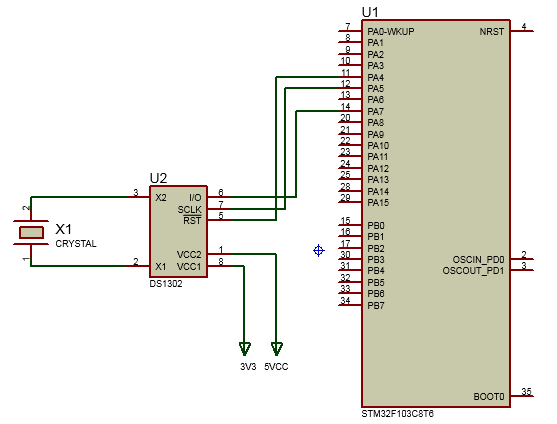
\includegraphics[scale=0.5]{Imagenes/DS1302_MCU_CONECTION.png}
\caption[Vista de las pistas de la cara delantera de la PCB tras el proceso de insolado]{Pistas PCB cara delantera}
\label{fig:001}
\end{figure}

\vspace{0.5cm}

\section{Configuración}
\subsection{STM CUBE MX}%------------------------------------------------------------------------------------------------------
Normalmente en la mayoría de proyectos solemos intentar que nuestro sistema vaya a la mayor velocidad posible, por ello trataremos de que nuestro sistema sea capaz de ejecutar las instrucciones lo mas rápido posible, para ello configuraremos la frecuencia del sistema a 72Mhz, que es la máxima que se puede alcanzar para este caso en concreto, dado que estamos hablando del STM32F103C8T6.
Para ello lo único que debemos hacer es aplicar las siguientes opciones el modo de configuración del RCC:

\begin{enumerate}
	\item Habilitar el HSE con la opción Crystal/ceramic resonator.Para ello es necesario disponer de un cristal de cuarzo de 8MHz conectado de forma externa, que , de serie ya incluye la placa de evaluación denominada "`Blue pill"'    
	\item Habilitar el LSE con la opción Crystal/ceramic resonator. Esta opción es recomendable aunque no necesaria, ésta habilita el cristal externo de 32khz para usar el RTC interno que dispone el microcontrolador. Si se requiere usar el TRC interno esta opciones indispensable.  
\end{enumerate}

\begin{figure}[H]
\centering
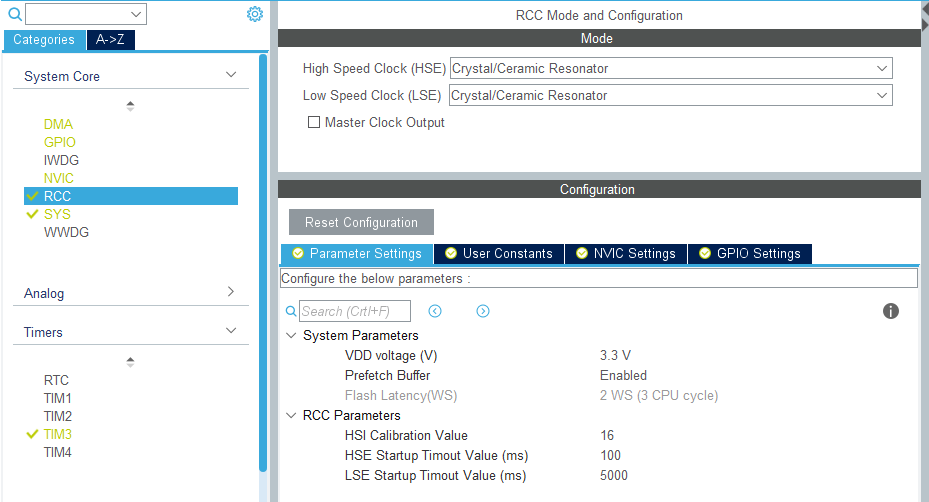
\includegraphics[scale=0.5]{Imagenes/Clock_CFG2.png}
\caption[Configuración de la frecuencia del sistema]{ }
\label{fig:002}
\end{figure}

\begin{figure}[H]
\centering
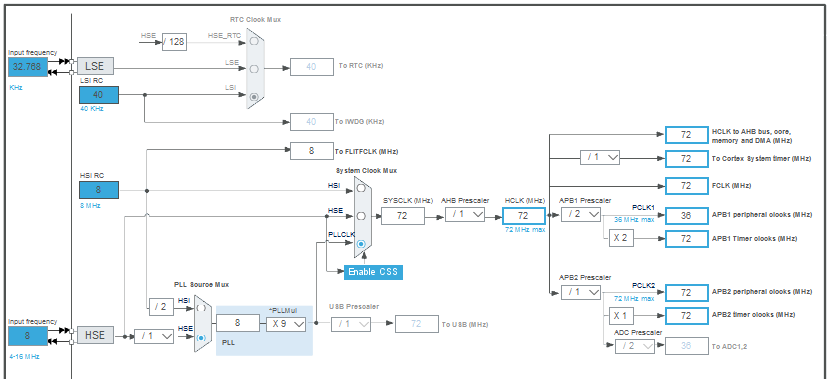
\includegraphics[scale=0.5]{Imagenes/Clock_CFG1.png}
\caption[Configuración de la frecuencia del sistema]{ }
\label{fig:003}
\end{figure}

Otra cosa muy importante es configurar un timer cada medio segundo, de esta forma nos aseguraremos de no perder ningún cambio en la variable de los segundos, una vez que salte el timer, se consultara al driver la fecha y la hora y se actualizaran las variables internas.

\begin{figure}[H]
\centering
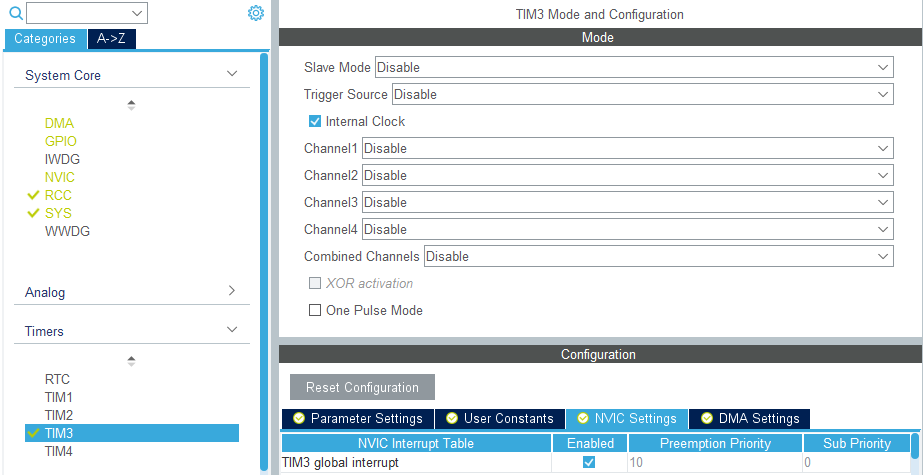
\includegraphics[scale=0.5]{Imagenes/TIMER3_CFG1.png}
\caption[Configuración de timer3 cada 500ms]{Configuración de timer3 cada 500ms}
\label{fig:004}
\end{figure}

\begin{figure}[H]
\centering
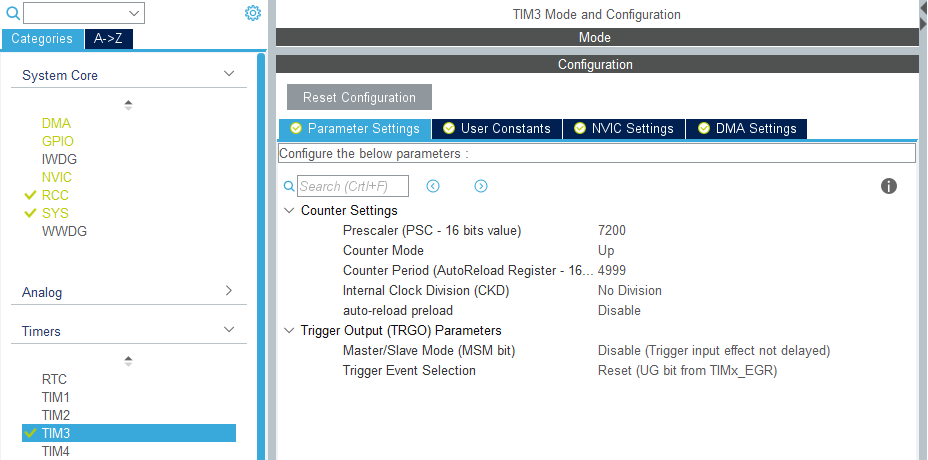
\includegraphics[scale=0.5]{Imagenes/TIMER3_CFG2.png}
\caption[Configuración de timer3 cada 500ms]{Configuración de timer3 cada 500ms}
\label{fig:005}
\end{figure}

Por supuesto, para flashear nuestro código en la placa necesitaremos configurar en nuestro sistema el modo JTAG 4 pin , de esta forma permitiremos el uso del STLINK V2 para el flashing /debug de nuestro código.

\begin{figure}[H]
\centering
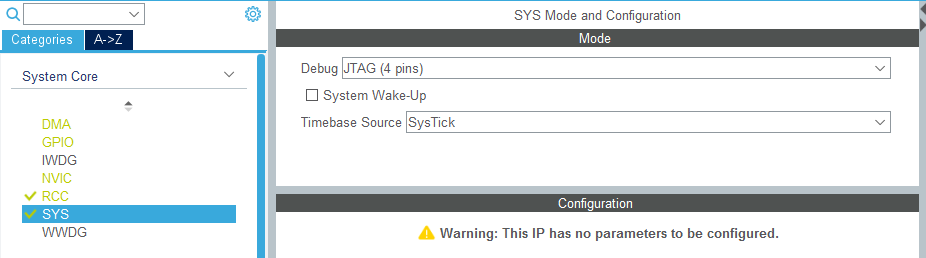
\includegraphics[scale=0.5]{Imagenes/JTAG_CFG.png}
\caption[Configuración del JTAG para el uso del STLINK-V2]{Configuración del JTAG para el uso del STLINK-V2}
\label{fig:006}
\end{figure}

El método mas sencillo para conocer que nuestro dispositivo esta funcionado correctamente es poder visualizar los valores que el dispositivo DS1302 le envía a nuestro microcontrolador, por ello se ha decidido usar un UART. continuara...  


\subsection{Programación del dispositivo}%------------------------------------------------------------------------------------------------------


\bigskip



\end{document}
